\documentclass[tikz,border=10pt]{standalone}
\usepackage{amsmath}
\usetikzlibrary{arrows.meta, positioning, calc, fit, decorations.pathreplacing}

\definecolor{c1}{HTML}{000000}
\definecolor{c2}{HTML}{233D4D}
\definecolor{c3}{HTML}{FE7F2D}
\definecolor{c4}{HTML}{EAECF0}
\definecolor{axiscolor}{HTML}{333333}
\definecolor{labelcolor}{HTML}{5F6B75}

\begin{document}
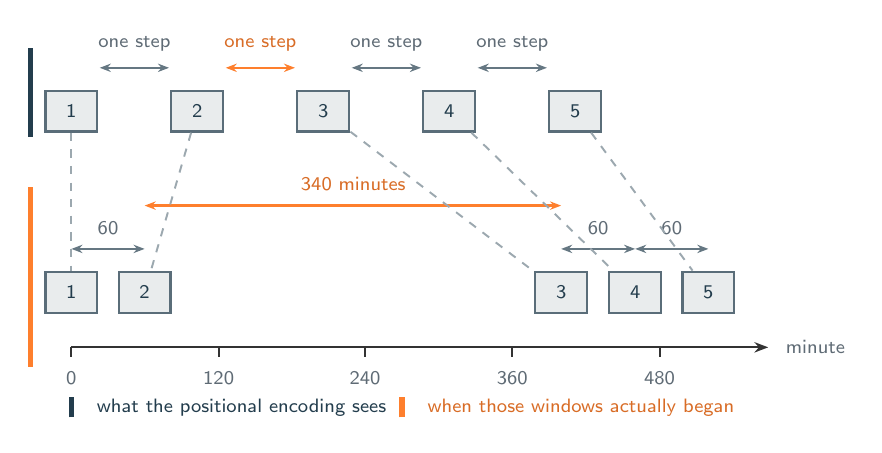
\begin{tikzpicture}[
    every node/.style={font=\sffamily},
    lab/.style={font=\sffamily\scriptsize, text=labelcolor},
    tag/.style={font=\sffamily\scriptsize, text=c2},
    hot/.style={font=\sffamily\scriptsize, text=c3!85!black},
    tok/.style={rectangle, draw=c2!75, fill=c2!10, line width=0.8pt,
                minimum width=0.66cm, minimum height=0.52cm,
                font=\sffamily\scriptsize, text=c2, inner sep=0pt},
    dbl/.style={{Stealth[length=4pt]}-{Stealth[length=4pt]}, line width=0.8pt},
    guide/.style={c2!45, line width=0.7pt, dashed},
]

% ================================================ side rules
\draw[c2, line width=2.0pt] (0.48, 5.35) -- (0.48, 4.22);
\draw[c3, line width=2.0pt] (0.48, 3.58) -- (0.48, 1.30);

% ================================================ what the encoding sees
\foreach \i/\x in {1/1.00, 2/2.60, 3/4.20, 4/5.80, 5/7.40}{
    \node[tok] (t\i) at (\x, 4.55) {\i};
}
\foreach \a/\b in {1.00/2.60, 4.20/5.80, 5.80/7.40}{
    \draw[dbl, c2!70] ({\a+0.36}, 5.10) -- ({\b-0.36}, 5.10);
    \node[lab, anchor=south] at ({(\a+\b)/2}, 5.18) {one step};
}
\draw[dbl, c3] (2.96, 5.10) -- (3.84, 5.10);
\node[hot, anchor=south] at (3.40, 5.18) {one step};

% ================================================ when they happened
\foreach \i/\x in {1/1.00, 2/1.93, 3/7.22, 4/8.16, 5/9.09}{
    \node[tok] (b\i) at (\x, 2.25) {\i};
}

\draw[axiscolor, line width=0.8pt, -{Stealth[length=5pt]}] (1.00, 1.55) -- (9.85, 1.55);
\foreach \m/\x in {0/1.00, 120/2.87, 240/4.73, 360/6.60, 480/8.47}{
    \draw[axiscolor, line width=0.7pt] (\x, 1.55) -- (\x, 1.43);
    \node[lab, anchor=north] at (\x, 1.37) {\m};
}
\node[lab, anchor=west] at (9.95, 1.55) {minute};

% the gaps, measured
\draw[dbl, c3] (1.93, 3.35) -- (7.22, 3.35);
\node[hot, anchor=south] at (4.58, 3.42) {340 minutes};
\foreach \a/\b in {1.00/1.93, 7.22/8.16, 8.16/9.09}{
    \draw[dbl, c2!70] (\a, 2.80) -- (\b, 2.80);
    \node[lab, anchor=south] at ({(\a+\b)/2}, 2.86) {60};
}

% the same token, top and bottom
\foreach \i in {1,2,3,4,5}{
    \draw[guide] (t\i) -- (b\i);
}

% ================================================ legend
\draw[c2, line width=2.0pt] (1.00, 0.66) -- (1.00, 0.92);
\node[tag, anchor=west] at (1.20, 0.79) {what the positional encoding sees};
\draw[c3, line width=2.0pt] (5.20, 0.66) -- (5.20, 0.92);
\node[hot, anchor=west] at (5.40, 0.79) {when those windows actually began};

\end{tikzpicture}
\end{document}
